



\documentclass[first=dgreen,second=purple,logo=yellowexc]{aaltoslides}
%\documentclass{aaltoslides} % DEFAULT
%\documentclass[first=purple,second=lgreen,logo=redque,normaltitle,nofoot]{aaltoslides} % SOME OPTION EXAMPLES





% input encode
\usepackage[utf8]{inputenc}


%\usepackage[T1]{fontenc}
%\usepackage{lastpage}
%\usepackage{multirow}
%\usepackage{colortbl}
%\usepackage{comment}
%\usepackage{bm}
%\usepackage{natbib}


% Lipsum package generates bullshit
%\usepackage{lipsum}

% Set the document languages
%\usepackage[finnish,swedish,english]{babel}

% nomenclature
%\usepackage[intoc]{nomencl}

% math
\usepackage{amsmath}

% bibliograph
%\usepackage{natbib}

% For algorithms
\usepackage{algorithm}
\usepackage{algorithmic}

% math font
\usepackage{amsfonts}

% theory
%\usepackage{amsthm}

% double bracket
\usepackage{stmaryrd}

% special math symbol
\usepackage{amssymb}

% use enumerate environment
%\usepackage{enumitem}

% use \url \hyperref, make reference clickable
\usepackage{hyperref}

% use lastpage to inde
\usepackage{lastpage}



%-------------------
%
% set
%
%-------------------
\newcommand{\Acal}{\mathcal{A}}
\newcommand{\Bcal}{\mathcal{B}}
\newcommand{\Ccal}{\mathcal{C}}
\newcommand{\Dcal}{\mathcal{D}}
\newcommand{\Ecal}{\mathcal{E}}
\newcommand{\Fcal}{\mathcal{F}}
\newcommand{\Gcal}{\mathcal{G}}
\newcommand{\Hcal}{\mathcal{H}}
\newcommand{\Ical}{\mathcal{I}}
\newcommand{\Jcal}{\mathcal{J}}
\newcommand{\Kcal}{\mathcal{K}}
\newcommand{\Lcal}{\mathcal{L}}
\newcommand{\Mcal}{\mathcal{M}}
\newcommand{\Ncal}{\mathcal{N}}
\newcommand{\Ocal}{\mathcal{O}}
\newcommand{\Pcal}{\mathcal{P}}
\newcommand{\Qcal}{\mathcal{Q}}
\newcommand{\Rcal}{\mathcal{R}}
\newcommand{\Scal}{\mathcal{S}}
\newcommand{\Tcal}{\mathcal{T}}
\newcommand{\Ucal}{\mathcal{U}}
\newcommand{\Vcal}{\mathcal{V}}
\newcommand{\Wcal}{\mathcal{W}}
\newcommand{\Xcal}{\mathcal{X}}
\newcommand{\Ycal}{\mathcal{Y}}
\newcommand{\Zcal}{\mathcal{Z}}

\newcommand{\RR}{\mathbb{R}}
\newcommand{\ZZ}{\mathbb{Z}}

%-------------------
%
% vector
%
%-------------------
\newcommand{\va}{\mathbf {a}}
\newcommand{\vb}{\mathbf {b}}
\newcommand{\vc}{\mathbf {c}}
\newcommand{\vd}{\mathbf {d}}
\newcommand{\ve}{\mathbf {e}}
\newcommand{\vf}{\mathbf {f}}
\newcommand{\vg}{\mathbf {g}}
\newcommand{\vh}{\mathbf {h}}
\newcommand{\vi}{\mathbf {i}}
\newcommand{\vj}{\mathbf {j}}
\newcommand{\vk}{\mathbf {k}}
\newcommand{\vl}{\mathbf {l}}
\newcommand{\vm}{\mathbf {m}}
\newcommand{\vn}{\mathbf {n}}
\newcommand{\vo}{\mathbf {o}}
\newcommand{\vp}{\mathbf {p}}
\newcommand{\vq}{\mathbf {q}}
\newcommand{\vr}{\mathbf {r}}
\newcommand{\vs}{\mathbf {s}}
\newcommand{\vt}{\mathbf {t}}
\newcommand{\vu}{\mathbf {u}}
\newcommand{\vv}{\mathbf {v}}
\newcommand{\vw}{\mathbf {w}}
\newcommand{\vx}{\mathbf {x}}
\newcommand{\vy}{\mathbf {y}}
\newcommand{\vz}{\mathbf {z}}
\newcommand{\vmu}{\mathbf {\mu}}
\newcommand{\valpha}{\mathbf {\alpha}}
\newcommand{\vlambda}{\mathbf {\lambda}}
\newcommand{\vAlpha}{\mathbf {\Alpha}}
\newcommand{\vbeta}{\mathbf {\beta}}
\newcommand{\vBeta}{\mathbf {\Beta}}
\newcommand{\vgamma}{\mathbf {\gamma}}
\newcommand{\vGamma}{\mathbf {\Gamma}}
\newcommand{\vdelta}{\mathbf {\dalta}}
\newcommand{\vDelta}{\mathbf {\Dalta}}
\newcommand{\vone}{\mathbf {1}}
\newcommand{\vzero}{\mathbf {0}}
\newcommand{\vell}{\mathbf {\ell}}
\newcommand{\vxi}{\mathbf{\xi}}
\newcommand{\vphi}{\mathbf{\phi}}
\newcommand{\vPhi}{\mathbf{\Phi}}

%-------------------
%
% math operation
%
%-------------------
\newcommand{\argmax}{\textbf{argmax}}
\newcommand{\argmin}{\textbf{argmin}}
\newcommand{\sign}{\textbf{sign}}
\newcommand{\maximize}{\textbf{max}}
\newcommand{\minimize}{\textbf{min}}
\newcommand{\argkmax}{\textbf{argkmax}}
\newcommand{\argkmin}{\textbf{argkmin}}
\newcommand{\kmaximize}{\textbf{kmax}}
\newcommand{\kminimize}{\textbf{kmin}}
\newcommand{\st}{\textbf{s.t.}}
\newcommand{\set}[1]{\{ #1 \}}
%\newcommand{\ind}[1]{{\llbracket #1 \rrbracket}}
\newcommand{\ind}[1]{\mathbf{1}_{\{#1\}}}
\newcommand{\norm}[1]{\left|\left| #1 \right|\right|}
\newcommand{\ip}[2]{\langle #1, #2 \rangle}
\newcommand{\var}{\textbf{Var}}
\newcommand{\E}{\textbf{E}}
\newcommand{\exponential}[1]{e^{ #1 }}


\newcommand{\Gva}{G_{\va}}
%-------------------
%
% writings
%
%-------------------
\newcommand{\eqdef}{\overset{{\rm \mbox{\tiny def}}}{=}}
\newcommand{\sbf}[1]{\boldsymbol{#1}}
\newcommand{\mbf}[1]{\mathbf{#1}} 
\newcommand{\etal}{{\em et al.}}

\newcommand{\svmstruct}{{\sc ssvm}}
\newcommand{\mmmn}{{\sc m$^3$n}}
\newcommand{\svm}{{\sc svm}}
\newcommand{\mmcrf}{{\sc mmcrf}}
\newcommand{\smo}{{\sc smo}}
\newcommand{\crf}{{\sc crf}}
\newcommand{\nphard}{$\Ncal\Pcal$-hard}
\newcommand{\nphardness}{$\Ncal\Pcal$-hardness}
\newcommand{\iis}{{\sc iis}}
\newcommand{\memm}{{\sc memm}}
\newcommand{\lr}{{\sc lr}}
\newcommand{\svmlight}{{\sc svmlight}}
\newcommand{\libsvm}{{\sc libsvm}}
\newcommand{\svmcascade}{{\sc svmcascade}}
\newcommand{\adaboost}{{\sc adaboost}}
\newcommand{\adaboostmh}{{\sc adaboost.mh}}
\newcommand{\bagging}{{\sc bagging}}
\newcommand{\vrtree}{{\sc vr-tree}}
\newcommand{\deepboosting}{{\sc deepboosting}}
\newcommand{\loo}{{\sc loo}}
\newcommand{\mtl}{{\sc mtl}}
\newcommand{\sdp}{{\sc sdp}}
\newcommand{\iqp}{{\sc iqp}}
\newcommand{\qp}{{\sc qp}}
\newcommand{\daggraph}{{\sc dag}}
\newcommand{\lp}{{\sc lp}}

\newcommand{\hatf}{{\hat{f}}}
\newcommand{\p}{\sc p}
\newcommand{\n}{\sc n}
\newcommand{\pp}{\sc pp}
\newcommand{\pn}{\sc pn}
\newcommand{\nn}{\sc nn}
\newcommand{\maxcut}{{\sc max-cut}}
\newcommand{\greedy}{{\sc greedy}}
\newcommand{\kernelcascade}{{\sc kernel cascade}}
\newcommand{\netrate}{{\sc netrate}}
\newcommand{\netinf}{{\sc netinf}}
\newcommand{\spin}{{\sc spin}}
\newcommand{\vI}{\mathbf{I}}
\newcommand{\tp}{^{\intercal}}
\newcommand{\mve}{{\sc mve}}
\newcommand{\amm}{{\sc amm}}
\newcommand{\mam}{{\sc mam}}
\newcommand{\rta}{{\sc rta}}
\newcommand{\lasso}{{\sc lasso}}
\newcommand{\mle}{{\sc mle}}
\newcommand{\map}{{\sc map}}
\newcommand{\rbf}{{\sc rbf}}
\newcommand{\mlknn}{{\sc ml-knn}}
\newcommand{\knn}{{\sc knn}}
\newcommand{\iblr}{{\sc iblr}}
\newcommand{\cc}{{\sc cc}}
\newcommand{\pcc}{{\sc pcc}}
\newcommand{\ecc}{{\sc ecc}}
\newcommand{\br}{{\sc br}}
\newcommand{\corrlog}{{\sc corrlog}}
\newcommand{\ilgs}{{\sc ilgs}}
\newcommand{\ilrs}{{\sc ilrs}}
\newcommand{\cpp}{{\sc c}}
\newcommand{\matlab}{{\sc matlab}}
\newcommand{\openmp}{{\sc openmp}}
\newcommand{\python}{{\sc python}}
\newcommand{\cvx}{{\sc cvx}}
\newcommand{\lda}{{\sc lda}}
\newcommand{\kkt}{{\sc k.k.t}}
\newcommand{\lbp}{{\sc lbp}}
\newcommand{\anova}{{\sc anova}}

\renewcommand{\algorithmicrequire}{\textbf{Input:}}
\renewcommand{\algorithmicensure}{\textbf{Output:}}



\newcommand{\Upsilonb}{\pmb \Upsilon}
\newcommand{\phib}{\pmb \phi}
\newcommand{\psib}{\pmb \psi}
\newcommand{\varphib}{\pmb \varphi}
\newcommand{\phibh}{\hat\phib}
\newcommand{\psibh}{\hat \psib}
\newcommand{\vYcal}{\pmb \Ycal}
\newcommand{\vXcal}{\pmb \Xcal}
\newcommand{\vFcal}{\pmb \Fcal}
%-------------------
%
% others
%
%-------------------




%\newtheorem{definition}{Definition}
%\newtheorem{theory}{Theory}
%\newtheorem{lemma}{Lemma}

















\title{Newton update in L$_2$-norm random tree approximation}
\author{Hongyu Su}



\institute[ICS]{
Helsinki Institute for Information Technology HIIT\\
Department of Computer Science\\
Aalto University
}

%\aaltofootertext{Random Spanning Tree Approximation}{\today}{\arabic{page}/\pageref{LastPage}\ }
\aaltofootertext{Newton update in \rta}{\today}{\arabic{page}}


\date{ \today} %\date{Version 1.0, \today}

\iffalse
\AtBeginSection[]
{
  \begin{frame}<beamer>{Outline}
    \tableofcontents[currentsection,subsection]
  \end{frame}
}
\fi




%--------------------------------
%
% document
%
%--------------------------------

\begin{document}


\aaltotitleframe
\footnotesize


\begin{frame}{Preliminaries}
	\begin{itemize}\footnotesize
		\item $\Xcal$ is an arbitrary input space, $\vx\in\vXcal$.
		\item $\Ycal$ is an output space of a set of $\ell$-dimensional {\em multilabels}
		\begin{align*}\footnotesize
			\vy=(y_1,\cdots,y_{\ell})\in\vYcal.
		\end{align*}
		\item $y_i$ is a {\em microlabel} and $y_i\in\{1,\cdots,r_i\}, r_i\in\ZZ$.
		\item For example, multilabel binary classification $y_i\in\{-1,+1\}$.
		\item Training examples are sampled from $(\vx,\vy)\in\vXcal\times\vYcal$.
		\item Each example $(\vx,\vy)$ is mapped into a joint feature space $\phib(\vx,\vy)$.
		\item $\vw$ is the weight vector in the joint feature space.
		\item Define a linear score function $F(\vw,\vx,\vy) = \ip{\vw}{\phib(\vx,\vy)}$.
		\item The prediction $\vy_{\vw}(\vx)$ of an input $\vx$ is the multilabel $\vy$ that maximizes the score function 
		\begin{align}\footnotesize
			\vy_{\vw}(\vx) = \underset{\vy\in\vYcal}{\argmax}\,\ip{\vw}{\phib(\vx,\vy)}. \label{inference}
		\end{align}
		\item (\ref{inference}) is called {\em inference} problem which is \nphard\ for most output feature maps.
	\end{itemize}
\end{frame}

\begin{frame}{Markov network}
	\begin{itemize}\footnotesize
		\item We assume that the joint feature map $\phib$ is a potential function on a Markov network $G=(E,V)$.
		\item $G$ is a complete graph with $|V| = \ell$ nodes and $|E| = \frac{\ell(\ell-1)}{2}$ undirected edges.
		\item $G$ models all pairwise correlations.
		\item $\varphib(\vx)$ is the input feature map, e.g., bag-of-words feature of an example $\vx$.
		\item $\psib(\vy)$ is the output feature map which is a collection of edges and labels
		\begin{align*}\footnotesize
			\varphib(\vy) = (u_{e})_{e\in E},u_e\in\{-1,+1\}^2.
		\end{align*}
		\item The joint feature is the Kronecker product of $\varphib(\vx)$ and $\psib(\vy)$
		\begin{align*}\footnotesize
			\phib(\vx,\vy) = (\phib_e(\vx,\vy))_{e\in E}=(\varphib(\vx)\otimes\psib_e(\vy_e))_{e\in E}.
		\end{align*}
		\item The score function can be factorized by the complete graph $G$
		\begin{align*}
			F(\vw,\vx,\vy) = \ip{\vw}{\phib(\vx,\vy)} = \sum_{e\in E}\ip{\vw_e}{\phib_e(\vx,\vy_e)}.
		\end{align*}
	\end{itemize}
\end{frame}

\begin{frame}{Inference in terms of all spanning trees}
	\begin{itemize}
		\item Solving the following inference problem on a complete graph is \nphard
		\begin{align*}
			\vy_{\vw}(\vx) = \underset{\vy\in\vYcal}{\argmax}\,F(\vw,\vx,\vy)  = \underset{\vy\in\vYcal}{\argmax}\,\sum_{e\in E}\ip{\vw_e}{\phib_e(\vx,\vy_e)}. 
		\end{align*}
		\item For a complete graph, there are $\ell^{\ell-2}$ unique spanning trees.
		\item We can write $F(\vw,\vx,\vy)$ as a conic combination of all spanning trees
		\begin{align*}
			F(\vw,\vx,\vy) &= \underset{T\in U(G)}{\E}a_T\ip{\vw_T}{\phib_T(\vx,\vy)}\\
			  &\underset{T\in U(G)}{\E}a_T^2=1,  \underset{T\in U(G)}{\E}a_T<1.
		\end{align*}
		\item $U(G)$ is the uniform distribution over $\ell^{\ell-2}$ spanning trees.
		\item The number of spanning trees is exponentially dependent on the number of nodes $\ell$.
	\end{itemize}
\end{frame}

\begin{frame}{A sample of $n$ spanning trees}
	\begin{itemize}\footnotesize
		\item Instead of using all spanning trees, we can just use $n$ spanning trees
		\begin{align*}\footnotesize
			F_{\Tcal}(\vw,\vx,\vy) &= \frac{1}{n}\sum_{i=1}^{n}a_{T_i}\ip{\vw_{T_i}}{\phib_{T_i}(\vx,\vy)}\\
			  &\frac{1}{n}\sum_{i=1}^{n}a_{T_i}^2=1,  \frac{1}{n}\sum_{i=1}^{n}a_{T_i}<1.
		\end{align*}
		\item When
		\begin{align*}\footnotesize
			n\ge\frac{\ell^2}{\epsilon^2}(\frac{1}{16}+\frac{1}{2}\ln\frac{8\sqrt{n}}{\delta}),
		\end{align*}
		we have $|F_{\Tcal}(\vw,\vx,\vy)-F(\vw,\vx,\vy)|\le\epsilon$, with high probability.
		\item A sample of $n\in\Theta(\ell^2/\delta^2)$ random spanning tree is sufficient to estimate the score function.
		\item Margin achieved by $F(\vw,\vx,\vy)$ is also preserved by the sample of $n$ random spanning trees $F_{\Tcal}(\vw,\vx,\vy)$.
	\end{itemize}
\end{frame}


\begin{frame}{Optimization problem}
	\begin{itemize}\footnotesize
		\item The primal optimization problem is defined as
		\begin{align*}\footnotesize
			\underset{\vw_{T_i},\xi_i}{\minimize} & \quad \frac{1}{2}\sum_{i=1}^{n}\norm{\vw_{T_i}}^2 + C\sum_{k=1}^{m}\xi_k\\
			\st & \quad \sum_{i=1}^{n}{ \langle \vw_{T_i}, \Delta\phib_{T_t}(\vx_k,\vy_k) \rangle}  \geq \ell_{T_i,k} -  \xi_k, \\
			& \quad \xi_k\ge0\, , \forall\ k \in \set{1,\dots,m}.
		\end{align*}
		\item The marginalized dual problem is defined as
		\begin{align*}\footnotesize
			\underset{\vmu\in\Mcal}{\maximize} & \quad \sum_{i=1}^{n}\left( \vmu_{T_i}\vell_{T_i} - \frac{1}{2}\vmu_{T_i}K^{\Delta\phib}_{T_i}\vmu_{T_i}\right)\\
			\st & \quad \sum_{u_e}\vmu_{T_i,e}(u_e)\le C.
		\end{align*}
	\end{itemize}
\end{frame}

\begin{frame}{Optimization on a single random spanning tree $T_i$}
	\begin{itemize}\footnotesize
		\item The optimization problem can be solved efficiently on a single tree $T_i$. 
		\item The algorithm iterates over all training examples until convergence.
		\item We drop the index momentarily $\mu\leftarrow\mu(j),\,g\leftarrow g(j),\,\ell\leftarrow\ell(j)$.
		\item For the $k$th iteration:
		\begin{enumerate}\footnotesize
			\item Obtain the current solution of the $j$th example $\vmu_{T_i}^k$.
			\item Compute the current gradient on $\vmu_{T_i}^k$, $g_{T_i}^k = \ell_{T_i} - K^{\Delta\phib}_{T_i}\vmu_{T_i}^k$.
			\item Compute a feasible solution ${\vmu}_{T_i}^{k,*}$ as an update direction ({\color{aaltored}efficiently})
			\begin{align}
				{\vmu}_{T_i}^{k,*} = \underset{\vmu\in\Mcal}{\argmax}\,\vmu\tp g_{T_i}^k. \label{tree_inference}
			\end{align}
			\item Compute an update direction from the current solution ${\vmu}_{T_i}^{k}$ towards the feasible solution ${\vmu}_{T_i}^{k,*}$
			\begin{align*}
				\Delta\vmu_{T_i}^{k} = {\vmu}_{T_i}^{k,*} - {\vmu}_{T_i}^{k}.
			\end{align*}
			\item Compute a stationary point ($\tau$) and perform the update
			\begin{align*}
				\vmu_{T_i}^{k+1} = \vmu_{T_i}^k + \tau\Delta\vmu_{T_i}^{k}.
			\end{align*}
		\end{enumerate}
	\end{itemize}
\end{frame}

\begin{frame}{Exact line search for a single tree}
	\begin{itemize}
		\item Line search gives the optimal feasible solution as a stationary point ($\tau$)
		\begin{align}
			\underset{\tau}{\maximize} &\quad f(\vmu_{T_i}^k + \tau\Delta\vmu_{T_i}^{k})\label{tree_line_search}\\
			\st &\quad 0\le\tau\le1.\nonumber
		\end{align}
		\item No update at $\tau=0$.
		\item Feasible maximum update is achieved at $\tau=1$. 
		\item The cost of (\ref{tree_line_search}) is significantly smaller than the cost of (\ref{tree_inference}).
	\end{itemize}
\end{frame}


\begin{frame}{Optimization on a collection of $n$ spanning trees}
	\begin{itemize}\footnotesize
		\item The algorithm iterates over all training examples until convergence.
		\item We drop the index momentarily $\mu\leftarrow\mu(j),\,g\leftarrow g(j),\,\ell\leftarrow\ell(j)$.
		\item For the $k$th iteration:
		\begin{enumerate}\footnotesize
			\item Obtain the current solutions over all spanning trees ${\color{aaltored}(}\vmu_{T_i}^k{\color{aaltored})_{i=1}^n}$.
			\item Compute the gradients over all trees ${\color{aaltored}(}g_{T_i}^k{\color{aaltored})_{i=1}^n}$.
			\item Compute a feasible solution for each individual spanning tree
			\begin{align*}
				{\vmu}_{T_i}^{k,*} = \underset{\vmu\in\Mcal}{\argmax}\,\vmu\tp g_{T_i}^k,\,{\color{aaltored}\forall i}.
			\end{align*}
			\item Compute the best feasible solution over the collection
			\begin{align*}
				{\vmu}_{T}^{k,*} = \underset{\vmu\in{\color{aaltored}(}{\vmu}_{T_i}^{k,*}{\color{aaltored})_{i=1}^n}}{\argmax}\,{\color{aaltored}\sum_{i=1}^n}\vmu\tp g_{T_i}^k
			\end{align*}
			\item Compute the update direction 
			\begin{align*}
				\Delta\vmu_{T_i}^{k} = {\vmu}_{T_i}^{k} - {\vmu}_{T}^{k,*},\,{\color{aaltored}\forall i}.
			\end{align*}
			\item Perform the update to the optimal feasible solution 
			\begin{align*}
				\vmu_{T_i}^{k+1} = \vmu_{T_i}^k + \tau\Delta\vmu_{T_i}^{k},\,{\color{aaltored}\forall i}.
			\end{align*}
		\end{enumerate}
	\end{itemize}
\end{frame}

\begin{frame}{Exact line search for the collection of trees}
	\begin{itemize}
		\item The step size along the update direction $\tau$ is given by the exact line search
		\begin{align*}\footnotesize
			\underset{\tau}{\maximize} &\quad {\color{aaltored}\sum_{i=1}^n}f(\vmu_{T_i}^k + \tau\Delta\vmu_{T_i}^{k})\\
			\st &\quad 0\le\tau\le1.
		\end{align*}
		\item Problems with the {\em best update}
		\begin{enumerate}\footnotesize
			\item The best feasible solution on a single tree might not be the best feasible solution on a collection of trees
			\begin{align*}
				{\vmu}_{T}^{k,*}\notin{\color{aaltored}(}{\vmu}_{T_i}^{k,*}{\color{aaltored})_{i=1}^n}.
			\end{align*}
			\item $\kappa$-best inference algorithm
			\begin{align*}
				({\vmu}_{T_i}^{k,*_h})_{h=1}^{\kappa} &= \underset{\vmu\in\Mcal}{\argmax}\,\vmu\tp g_{T_i}^k,\,{\color{aaltored}\forall i}\\
				{\vmu}_{T}^{k,*} &\in {\color{aaltored}(}{\vmu}_{T_i}^{k,*_h}{\color{aaltored})_{i=\{1,\cdots,n\},h\in\{1,\cdots,\kappa\}}}.
			\end{align*}
		\end{enumerate}
	\end{itemize}
\end{frame}

\begin{frame}{Update with multiple directions}
	\begin{itemize}\footnotesize
		\item The algorithm iterates over all training examples until convergence.
		\item We drop the index momentarily $\mu\leftarrow\mu(j),\,g\leftarrow g(j),\,\ell\leftarrow\ell(j)$.
		\item For the $k$th iteration:
		\begin{enumerate}\footnotesize
			\item Obtain the current solutions over all spanning trees ${\color{aaltored}(}\vmu_{T_i}^k{\color{aaltored})_{i=1}^n}$.
			\item Compute the gradients over all trees ${\color{aaltored}(}g_{T_i}^k{\color{aaltored})_{i=1}^n}$.
			\item Compute a feasible solution for each individual spanning tree
			\begin{align*}
				{\vmu}_{T_i}^{k,*} = \underset{\vmu\in\Mcal}{\argmax}\,\vmu\tp g_{T_i}^k,\,{\color{aaltored}\forall i}.
			\end{align*}
			\item Project each local feasible solution to a global feasible solution
			\begin{align*}
				{\vmu}_{T_i}^{G,k,*} \leftarrow {\vmu}_{T_i}^{k,*},\,{\color{aaltored}\forall i}.
			\end{align*}
			\item Define a conic combination of update directions 
			\begin{align*}
				\Delta{\vmu}^{G,k} = \sum_{i=1}^{n}\tau_i \Delta{\vmu}_{T_i}^{G,k,*} = \sum_{i=1}^{n}\tau_i \left({\vmu}^{G,k} -{\vmu}_{T_i}^{G,k,*}\right), 0\le\tau_i\le1,\forall i.
			\end{align*}
			\item Perform the update $\vmu^{G,k+1} = \vmu^{G,k} + \Delta{\vmu}^{G,k+1}.$
			\item Project the global solution on spanning trees ${\color{aaltored}(}\vmu_{T_i}^{k+1}{\color{aaltored})_{i=1}^n}{\leftarrow}\vmu^{G,k+1}.$
		\end{enumerate}
	\end{itemize}
\end{frame}


\begin{frame}{Newton method to compute $\vtau$}
	\begin{itemize}\footnotesize
		\item We want to find $\tau$ that maximize the objective function given the update
		% \begin{align*}\footnotesize
		% 	&f(\vmu^{G,k} + \Delta{\vmu}^{G,k+1}) \\
		% 	&= (\vmu^{G,k} + \Delta{\vmu}^{G,k+1})\tp\ell_G - \frac{1}{2}(\vmu^{G,k} + \Delta{\vmu}^{G,k+1})\tp K_G (\vmu^{G,k} + \Delta{\vmu}^{G,k+1}).
		% \end{align*}
		\begin{align*}
			\underset{\tau}{\maximize} & \quad f(\vmu^{G,k} + \Delta{\vmu}^{G,k+1})\\
			\st & \quad 0\le\tau_i\le1.
		\end{align*}
		\item The objective is quadratic with respect to $\vtau$.
		\item We use Newton method to find $\vtau$ that maximize the objective.
		\item $\vtau$ is projected into the feasible region.
	\end{itemize}
\end{frame}


\begin{frame}{Compute duality gap}
	\begin{itemize}\footnotesize
		\item We use duality gap to measure the progress of the optimization.
		\item Primal and dual objective function
		\begin{align*}\footnotesize
			f(\vw) &= \frac{1}{2}||\vw||^2 + C\sum_{i=1}^m\left(\ell_i-\ip{\vw}{\Delta\phib(\vx_i,\vy_i)}\right)\\
			g(\valpha) &= \sum_{i=1}^m\alpha_i\ell_i - \frac{1}{2}\sum_{i=1}^m\sum_{j=1}^m\alpha_iK^{\Delta\phib}(\vx_i,\vy_i;\vx_j,\vy_j)\alpha_j
		\end{align*}
		\item $\underset{\valpha}{\maximize}\,g(\valpha)\le \underset{\vw}{\minimize}\,f(\vw)$, minimum gap when optimal.
		\item Duality gap at $\valpha^k$
		\begin{align*}\footnotesize
			f(\vw^k) - g(\valpha^k) &= C\left(\vell-K^{\Delta\phib}\valpha^k\right) - \valpha^k\left(\vell-K^{\Delta\phib}\valpha^k\right)\\
			&= C\tp \nabla g(\valpha^k) -{\valpha^k} \tp \nabla g(\valpha^k)
		\end{align*}
	\end{itemize}
		\begin{enumerate}\footnotesize
			\item Estimate the dual objective function using a linear approximation $\nabla g$.
			\item Dual objective value at $\valpha^k$ is computed by ${\valpha^k} \tp \nabla g(\valpha^k)$.
			\item Primal objective value is estimate by $C\tp \nabla g(\valpha^k)$.
		\end{enumerate}
\end{frame}


\begin{frame}{Experimental results - Objective value}
	\only<1>{
	\begin{itemize}\footnotesize
		\item Compare update with the best direction v.s. update with multiple directions
		\item Number of spanning trees $|T|=\{5,10,20\}$.
		\item Each spanning tree outputs top $\kappa=1$ best direction.
	\end{itemize}
	\begin{figure}
		\begin{center}
			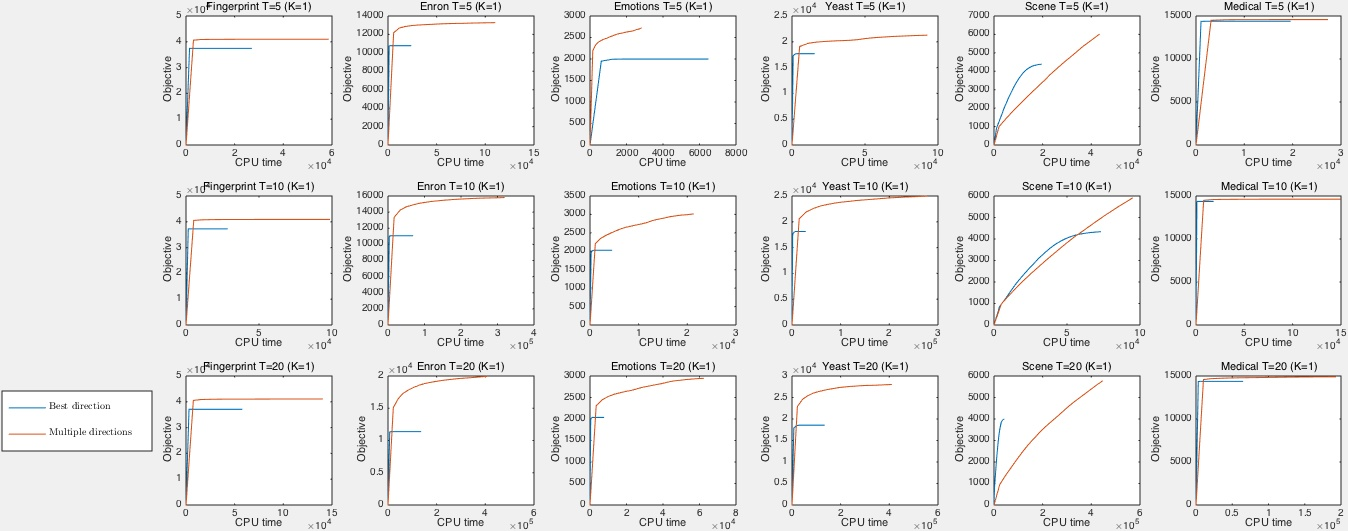
\includegraphics[scale=0.22]{./slide_objective_k1.jpg}
		\end{center}
	\end{figure}}
	\only<2>{
	\begin{itemize}\footnotesize
		\item Compare update with the best direction v.s. update with multiple directions
		\item Number of spanning trees $|T|=\{5,10,20\}$.
		\item Each spanning tree outputs top $\kappa=10$ best directions.
	\end{itemize}
	\begin{figure}
		\begin{center}
			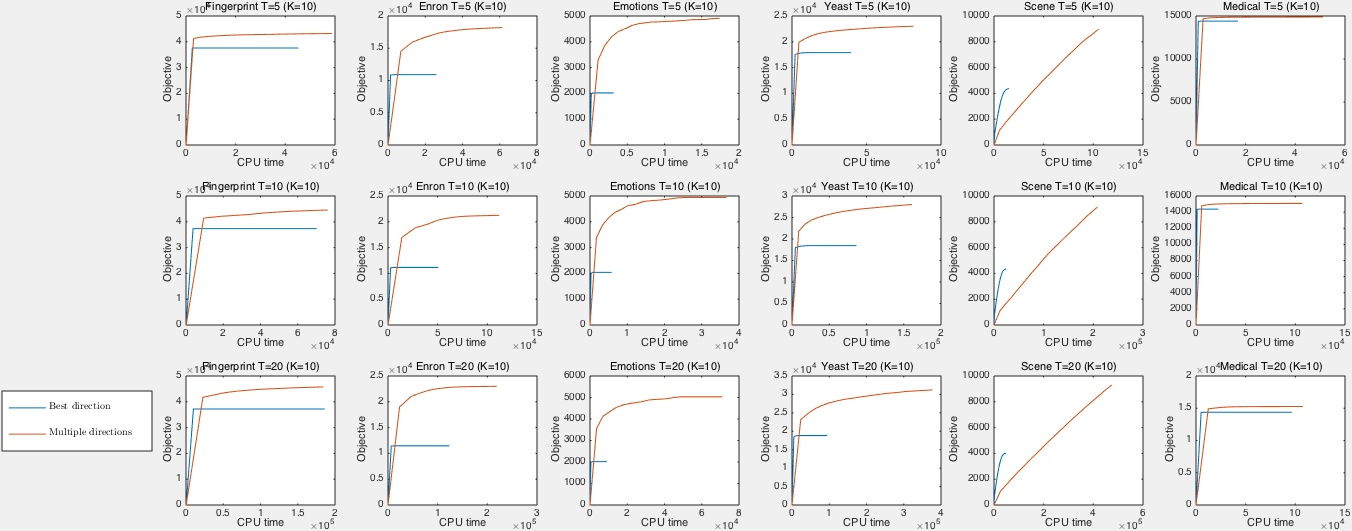
\includegraphics[scale=0.22]{./slide_objective_k10.jpg}
		\end{center}
	\end{figure}
	}
\end{frame}

\begin{frame}{Experimental results - Duality gap}
	\only<1>{
	\begin{itemize}\footnotesize
		\item Compare update with the best direction v.s. update with multiple directions
		\item Number of spanning trees $|T|=\{5,10,20\}$.
		\item Each spanning tree outputs top $\kappa=1$ best direction.
	\end{itemize}
	\begin{figure}
		\begin{center}
			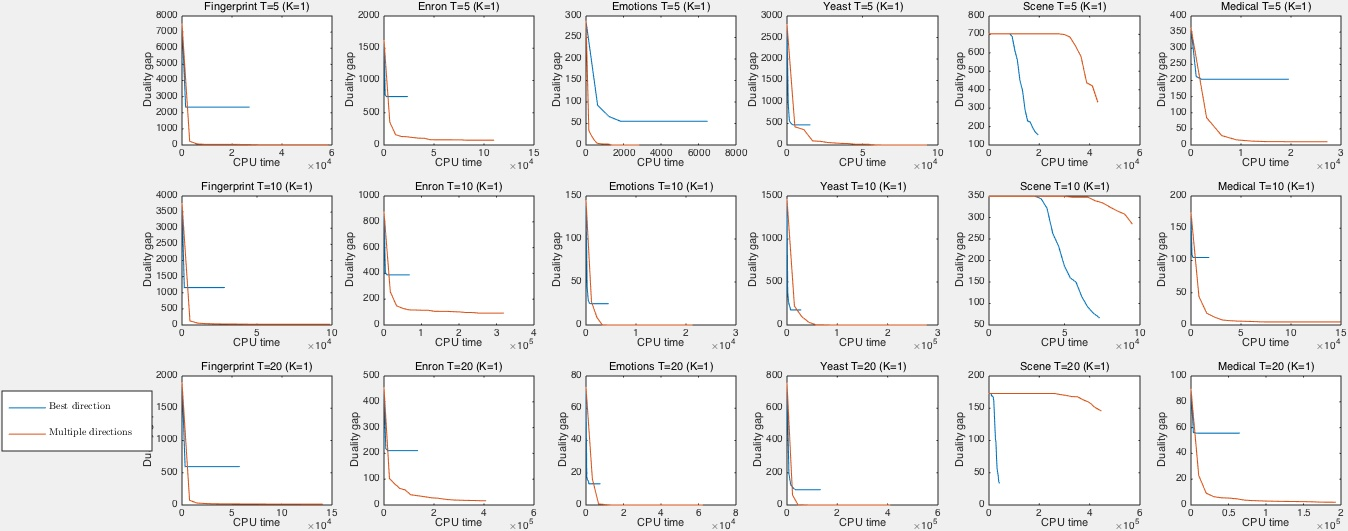
\includegraphics[scale=0.22]{./slide_duality_gap_value_k1.jpg}
		\end{center}
	\end{figure}}
	\only<2>{
	\begin{itemize}\footnotesize
		\item Compare update with the best direction v.s. update with multiple directions
		\item Number of spanning trees $|T|=\{5,10,20\}$.
		\item Each spanning tree outputs top $\kappa=10$ best directions.
	\end{itemize}
	\begin{figure}
		\begin{center}
			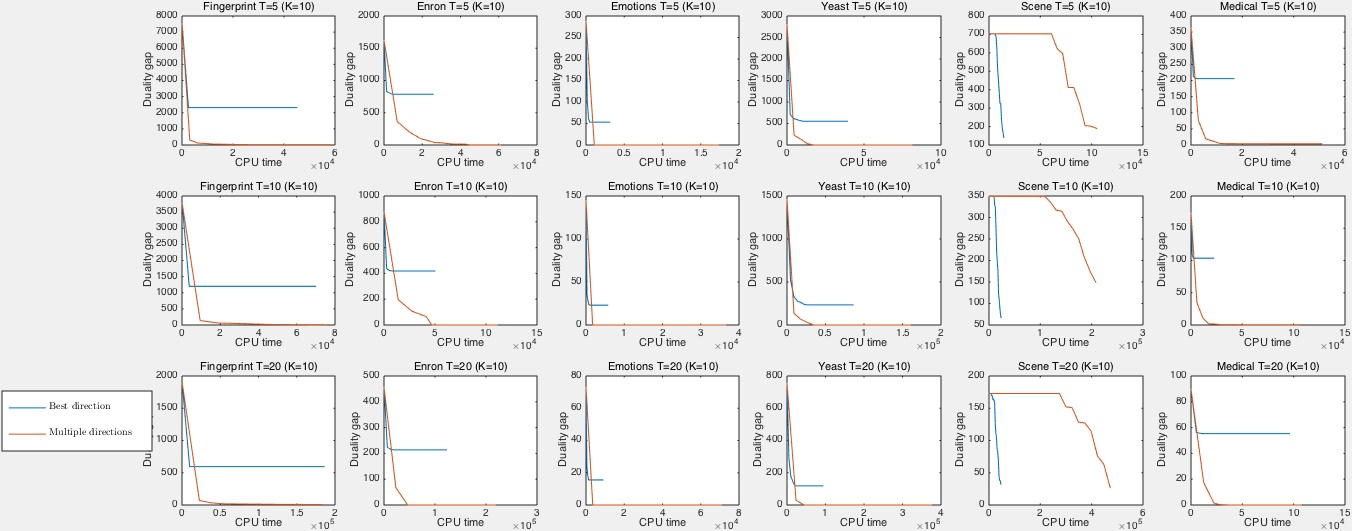
\includegraphics[scale=0.22]{./slide_duality_gap_value_k10.jpg}
		\end{center}
	\end{figure}
	}
\end{frame}

\begin{frame}{Experimental results - Relative duality gap}
	\only<1>{
	\begin{itemize}\footnotesize
		\item Compare update with the best direction v.s. update with multiple directions
		\item Number of spanning trees $|T|=\{5,10,20\}$.
		\item Each spanning tree outputs top $\kappa=1$ best direction.
	\end{itemize}
	\begin{figure}
		\begin{center}
			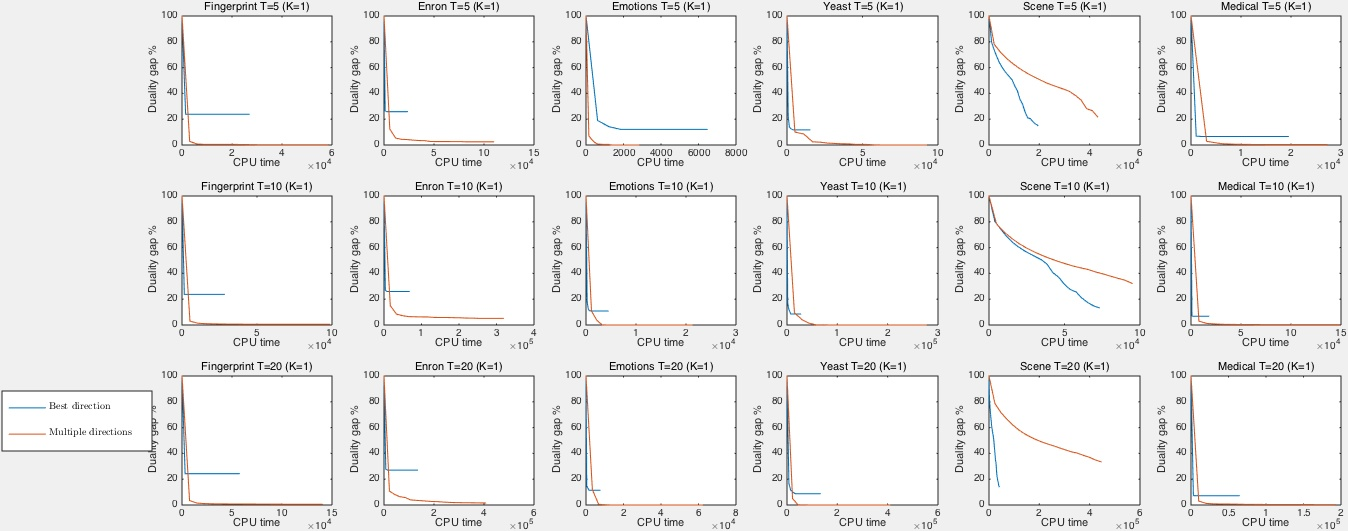
\includegraphics[scale=0.22]{./slide_duality_gap_percentage_k1.jpg}
		\end{center}
	\end{figure}}
	\only<2>{
	\begin{itemize}\footnotesize
		\item Compare update with the best direction v.s. update with multiple directions
		\item Number of spanning trees $|T|=\{5,10,20\}$.
		\item Each spanning tree outputs top $\kappa=10$ best directions.
	\end{itemize}
	\begin{figure}
		\begin{center}
			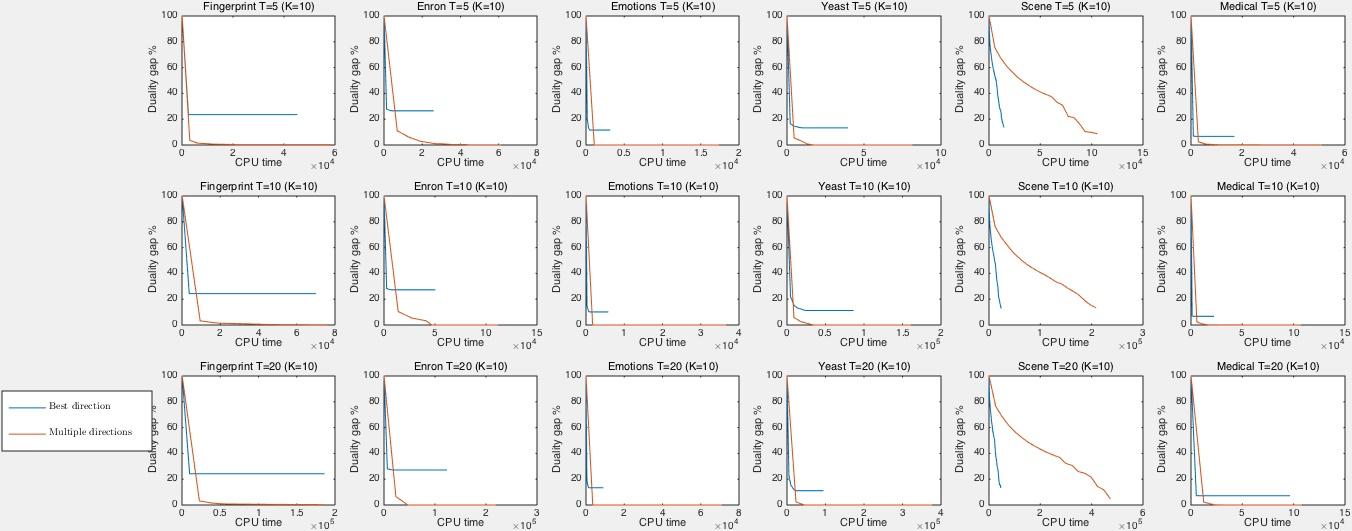
\includegraphics[scale=0.22]{./slide_duality_gap_percentage_k10.jpg}
		\end{center}
	\end{figure}
	}
\end{frame}


\begin{frame}{Experimental results - Hamming loss training}
	\only<1>{
	\begin{itemize}\footnotesize
		\item Compare update with the best direction v.s. update with multiple directions
		\item Number of spanning trees $|T|=\{5,10,20\}$.
		\item Each spanning tree outputs top $\kappa=1$ best direction.
	\end{itemize}
	\begin{figure}
		\begin{center}
			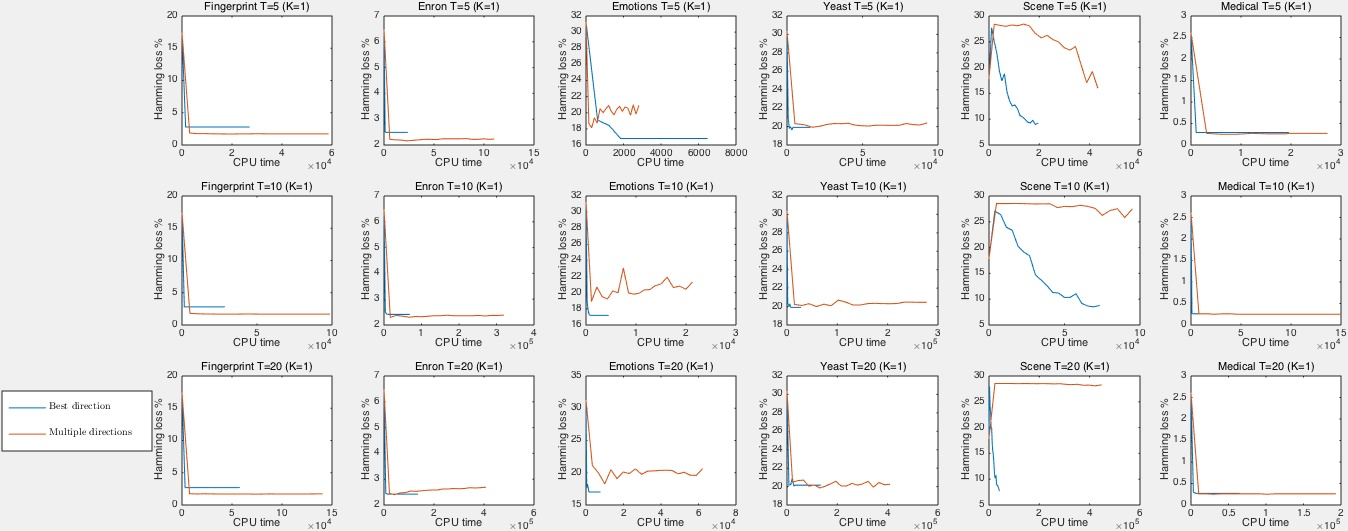
\includegraphics[scale=0.22]{./slide_hamming_loss_k1.jpg}
		\end{center}
	\end{figure}}
	\only<2>{
	\begin{itemize}\footnotesize
		\item Compare update with the best direction v.s. update with multiple directions
		\item Number of spanning trees $|T|=\{5,10,20\}$.
		\item Each spanning tree outputs top $\kappa=10$ best directions.
	\end{itemize}
	\begin{figure}
		\begin{center}
			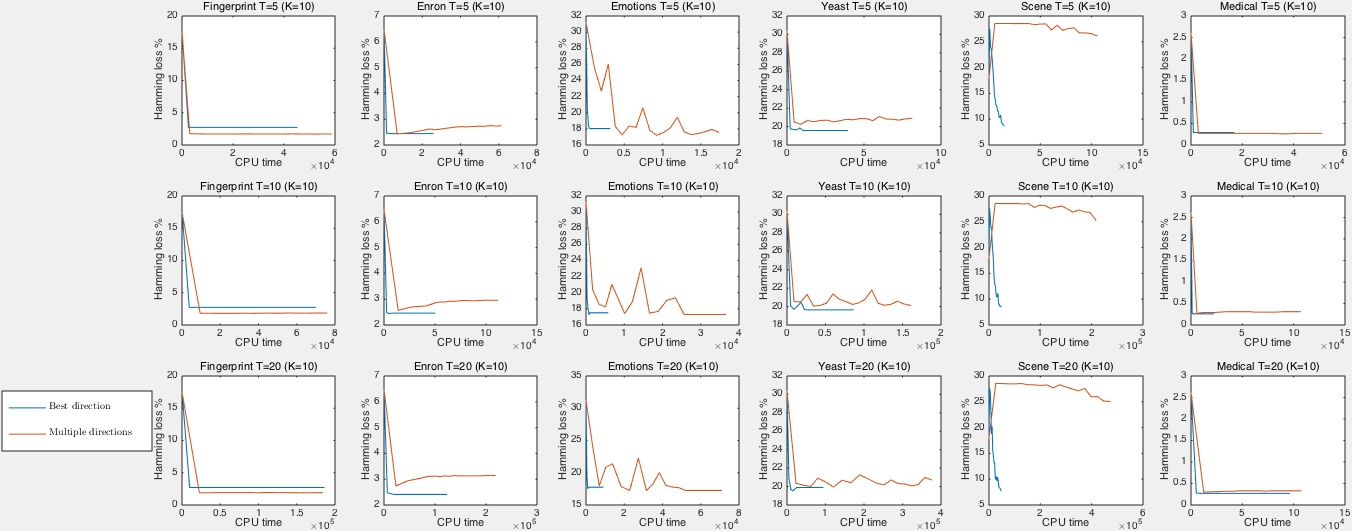
\includegraphics[scale=0.22]{./slide_hamming_loss_k10.jpg}
		\end{center}
	\end{figure}
	}
\end{frame}

\begin{frame}{Experimental results}
	\begin{itemize}\footnotesize
		\item Number of spanning trees $|T|=\{5,10,20\}$.
		\item Each spanning tree outputs $\kappa=\{1,\cdots,16\}$ best directions.
	\end{itemize}
	\begin{figure}
		\begin{center}
			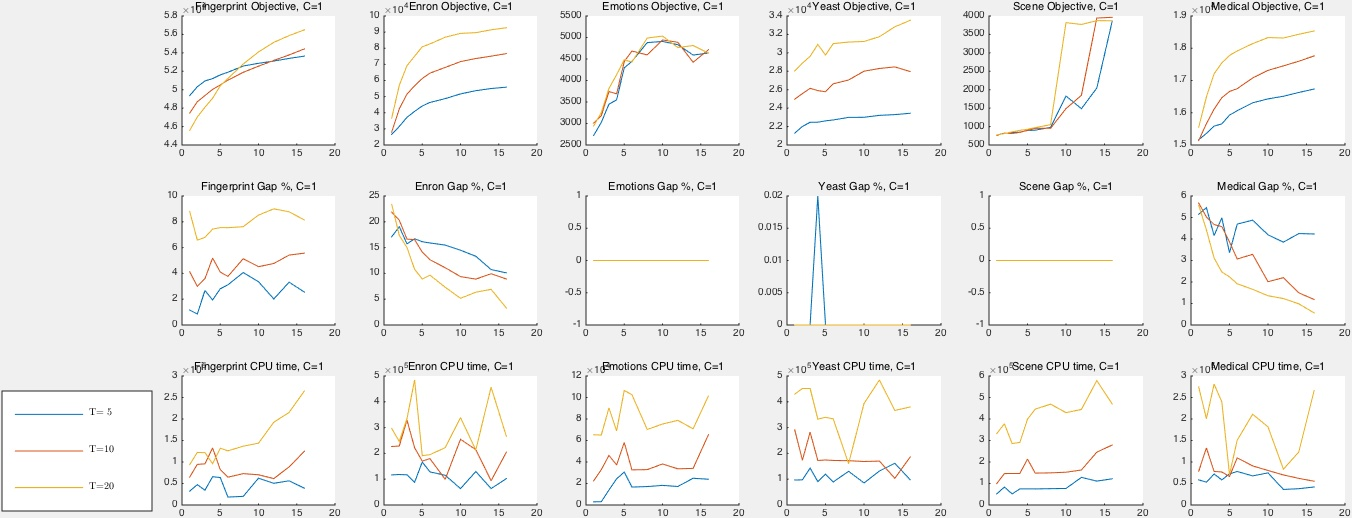
\includegraphics[scale=0.22]{./slide_overall_objective.jpg}
		\end{center}
	\end{figure}
\end{frame}

\begin{frame}{Experimental results}
	\begin{itemize}\footnotesize
		\item Number of spanning trees $|T|=\{5,10,20\}$.
		\item Each spanning tree outputs $\kappa=\{1,\cdots,16\}$ best directions.
	\end{itemize}
	\begin{figure}
		\begin{center}
			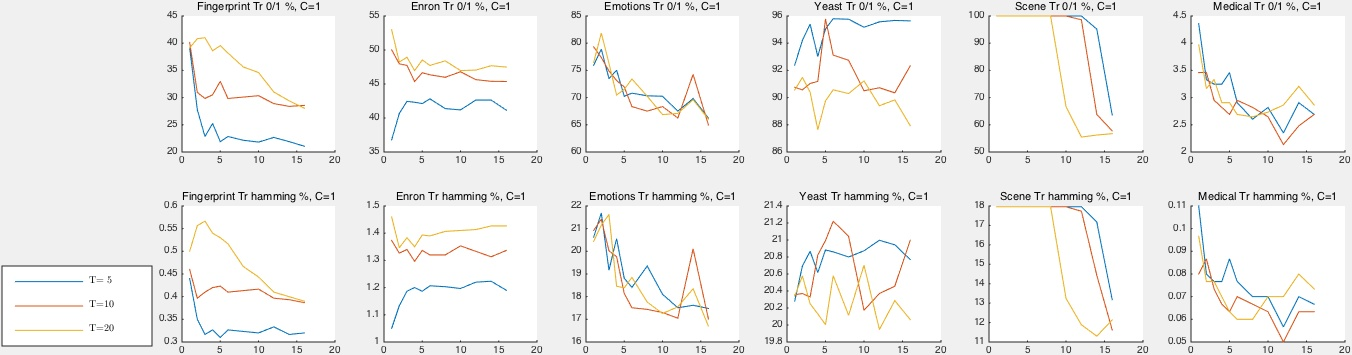
\includegraphics[scale=0.22]{./slide_overall_training.jpg}
		\end{center}
	\end{figure}
\end{frame}

\begin{frame}{Experimental results}
	\begin{itemize}\footnotesize
		\item Number of spanning trees $|T|=\{5,10,20\}$.
		\item Each spanning tree outputs $\kappa=\{1,\cdots,16\}$ best directions.
	\end{itemize}
	\begin{figure}
		\begin{center}
			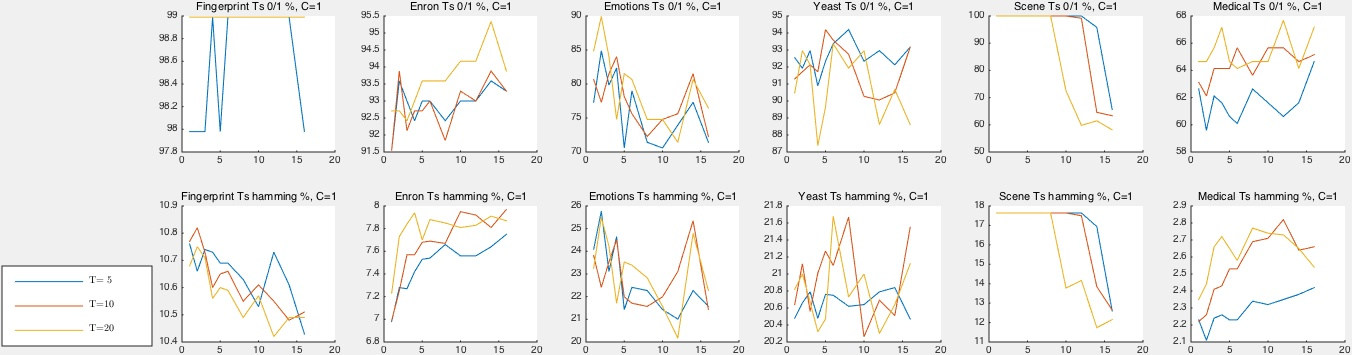
\includegraphics[scale=0.22]{./slide_overall_test.jpg}
		\end{center}
	\end{figure}
\end{frame}


% \begin{frame}{}
% 	\begin{itemize}
% 	\end{itemize}
% \end{frame}


% \begin{frame}{}
% 	\begin{itemize}
% 	\end{itemize}
% \end{frame}


%
\begin{frame}{Conclusions}
	\begin{itemize}\footnotesize
		\item 
	\end{itemize}
\end{frame}




\iffalse
\begin{frame}[allowframebreaks]{Bibliography}
	%\bibliographystyle{plain}
	\bibliographystyle{apalike}
	\bibliography{example}
\end{frame}
\fi


\end{document}
